\documentclass[a4paper,ngerman,12pt]{exam}
\usepackage{babel}
\usepackage[utf8]{inputenc}
\usepackage[T1]{fontenc}
\usepackage{graphicx}
\usepackage{algpseudocode}
\usepackage{geometry}
\usepackage{csquotes} % Anführungszeichen
\usepackage{paralist} % kompakte Aufzählungen
\usepackage{textcomp,tikz} %diverses
\usepackage{amsmath,amssymb,amstext,amsthm}
\usepackage{listings}
\usepackage{mathtools}
\usepackage{mdframed} % Boxen
\usepackage{float}
\usepackage{tikz}
\usetikzlibrary{calc}
\usetikzlibrary{arrows, automata}

\geometry{a4paper, top=3cm, left=2.7cm, right=2.7cm}
\pagestyle{plain}
\renewcommand{\solutiontitle}{\noindent\textbf{Lösung:}\enspace}
\DeclarePairedDelimiter\ceil{\lceil}{\rceil}
\DeclarePairedDelimiter\floor{\lfloor}{\rfloor}

%\printanswers

\begin{document}
\noindent Theoretische Informatik \hfill Gruppe 8 \\
\mbox{}\hfill Loris Reiff
\begin{center}
  \bfseries\Large
  Quiz 3\ifprintanswers
  -- Lösungen
\fi
\end{center}

\begin{questions}
  \question Betrachte folgenden EA.

  \begin{figure}[h]
    \centering
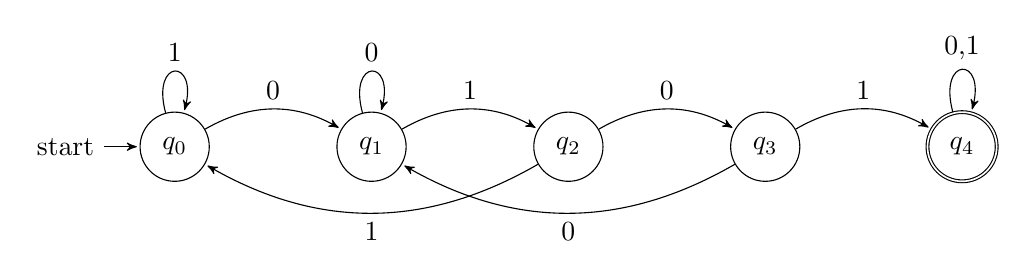
\begin{tikzpicture}[->,>=stealth',shorten >=1pt,auto,node distance=2.5cm]
  \node[initial, state]   (q0)                {$q_0$};
  \node[state]            (q1) [right of=q0]  {$q_1$};
  \node[state]            (q2) [right of=q1]  {$q_2$};
  \node[state]            (q3) [right of=q2]  {$q_3$};
  \node[state, accepting] (q4) [right of=q3]  {$q_4$};

  \path[->]
        (q0) edge [bend left]  node [above] {0} (q1)
             edge [loop above] node [above] {1} (q0)
        (q1) edge [loop above] node [above] {0} (q1)
             edge [bend left]  node [above] {1} (q2)
        (q2) edge [bend left]  node [above] {0} (q3)
             edge [bend left]  node [below] {1} (q0)
        (q3) edge [bend left]  node [below] {0} (q1)
             edge [bend left]  node [above] {1} (q4)
        (q4) edge [loop above] node [above] {0,1} (q4);
\end{tikzpicture}
  \end{figure}

  Welche Aussagen sind korrekt?
  \begin{checkboxes}
    \CorrectChoice $\text{Kl}[q_0] = \{\lambda, 1\} \cup \{x \in \{0, 1\}^* \mid
      \text{ endet mit } 11
      \text{ und enthält nicht das Teilwort } 0101\}$
  \choice $\text{Kl}[q_1] = \{x \in \{0, 1\}^* \mid x \text{ endet mit } 0
      \text{ und beinhaltet nicht das Teilwort } 0101\}$
  \CorrectChoice $\text{Kl}[q_2] = \{x \in \{0, 1\}^* \mid x \text{ endet mit } 01
      \text{ und enthält nicht das Teilwort } 0101\}$
  \choice $\text{Kl}[q_3] = \{x \in \{0, 1\}^* \mid x \text{ endet mit } 010
      \text{ und enthält nicht das Teilwort } 10101\} $
  \choice $\text{Kl}[q_4] = \{x \in \{0, 1\}^* \mid
         x \text{ enthält das Teilwort } 10101\}$
  \CorrectChoice $\text{Kl}[q_4] = \{x \in \{0, 1\}^* \mid
         x \text{ enthält das Teilwort } 0101\}$
  \end{checkboxes}
    \begin{solution} $ $\\
      $010 \in \{x \in \{0, 1\}^* \mid x \text{ endet mit } 0
      \text{ und beinhaltet nicht das Teilwort } 0101\}$ aber $010 \not\in \text{Kl}[q_1]$

$0101 \in \{x \in \{0, 1\}^* \mid x \text{ endet mit } 010
      \text{ und enthält nicht das Teilwort } 10101\}$ aber
      $0101 \not\in \text{Kl}[q_3]$
    \end{solution}

  \question
  \begin{parts}
    \part
  Entwerfe einen endlichen Automaten (in Diagrammdarstellung) für folgende Sprache:
  \begin{align*}
    L &= \{w \in \{a,b, c\}^* \mid (|w|_a + 2|w|_b) \bmod 3 \equiv 1\}
  \end{align*}

    \begin{solutionorbox}[17em]
\begin{figure}[H]
  \label{fig:l1}
  \centering
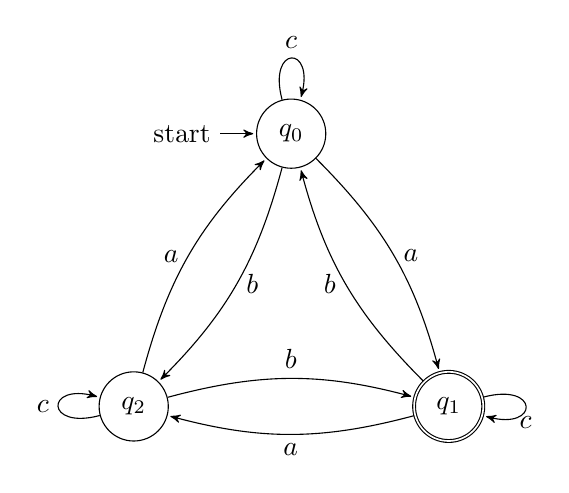
\begin{tikzpicture}[->,>=stealth',shorten >=1pt,auto,node distance=2.5cm]
  \node[initial, state]   (q0)                {$q_{0}$};
  \node[state, accepting] (q1) at ($ (q0) + (-60:4) $) {$q_{1}$};
  \node[state]            (q2) at ($ (q0) + (-120:4)$) {$q_{2}$};

  \path[->]
        (q0) edge [bend left=15]  node [right] {$a$} (q1)
        (q1) edge [bend left=15]  node [below] {$a$} (q2)
        (q2) edge [bend left=15]  node [left]  {$a$} (q0)

        (q1) edge [bend left=15]  node [left]  {$b$} (q0)
        (q2) edge [bend left=15]  node [above] {$b$} (q1)
        (q0) edge [bend left=15]  node [right] {$b$} (q2)

        (q0) edge [loop above]  node [above] {$c$} (q0)
        (q1) edge [loop right]  node [below] {$c$} (q1)
        (q2) edge [loop left]  node [left] {$c$} (q2);
\end{tikzpicture}
\end{figure}
    \end{solutionorbox}
  \part
    Gib die Klassen Kl[$q$] für jeden Zustand $q$ an:
    \begin{solutionorbox}[4em]
     $\text{Kl}[q_i] = \{w \in \{a,b,c\}^* \mid (|w|_a + 2|w|_b) \bmod 3 \equiv i\}$
    \end{solutionorbox}
  \end{parts}

  \question
  Entwerfe einen endlichen Automaten (in Diagrammdarstellung) mit
  möglichst wenig Zuständen für folgende Sprache:
  \begin{align*}
    L &= \{0, 01, 101, 10001\} \subseteq \{0,1\}^*
  \end{align*}
    \begin{solutionorbox}[17em]
\begin{figure}[H]
  \centering
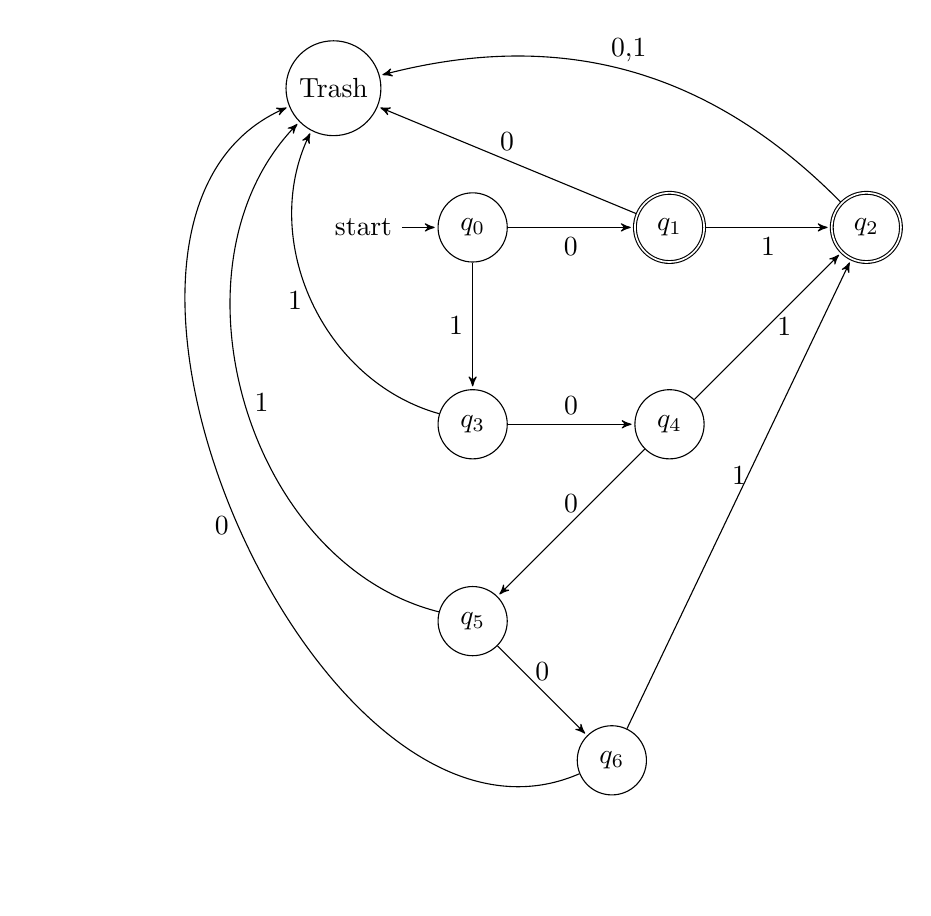
\begin{tikzpicture}[->,>=stealth',shorten >=1pt,auto,node distance=2.5cm]
  \node[initial, state]   (q0)                {$q_0$};
  \node[state, accepting] (q1) [right of=q0]  {$q_1$};
  \node[state, accepting] (q2) [right of=q1]  {$q_2$};
  \node[state]            (q3) [below of=q0]  {$q_3$};
  \node[state]            (q4) [right of=q3]  {$q_4$};
  \node[state]            (q5) [below of=q3]  {$q_5$};
  \node[state]            (q6) [below right of=q5]  {$q_6$};
  \node[state]            (t)  [above left of=q0]  {Trash};

  \path[->]
        (q0) edge [] node [below] {0} (q1)
             edge [] node [left]  {1} (q3)
        (q1) edge [] node [above] {0} (t)
             edge [] node [below] {1} (q2)
        (q2) edge [bend right] node [above] {0,1} (t)
        (q3) edge [] node [above] {0} (q4)
             edge [bend left=50]  node [left] {1} (t)
        (q4) edge [] node [above] {0} (q5)
             edge [] node [right]  {1} (q2)
        (q5) edge [] node [above] {0} (q6)
             edge [bend left=60] node [right] {1} (t)
        (q6) edge [] node [above] {1} (q2)
             edge [bend left=90] node [left] {0} (t);
\end{tikzpicture}
\end{figure}
    \end{solutionorbox}

\end{questions}

\end{document}
